\section{Experiments}

\subsection{Setup}

Each solver was run once on each test stage, starting from the stage's initial state. The runs
are produced by \texttt{experiments/run\_experiments.py}, which writes
\texttt{experiments/summary\_4\_metrics.csv}; the charts are drawn from that file by
\texttt{experiments/plot\_results.py} (pandas, matplotlib and seaborn). The algorithms are
deterministic: re-running the experiment reproduces exactly the same expanded nodes, solution
lengths and paths. Search time and memory depend on the machine, and time is inflated several times
by \texttt{tracemalloc}, so they are meaningful only \emph{relative to each other}.

\begin{table}[H]
\centering
\caption{Measured quantities}
\label{tab:metrics}
\begin{tabularx}{\linewidth}{llX}
\toprule
\textbf{Metric} & \textbf{Unit} & \textbf{How it is measured} \\
\midrule
Search time & ms & \texttt{time.perf\_counter()} around the search loop \\
Memory usage & KB & Peak traced allocation during the search (\texttt{tracemalloc}) \\
Expanded nodes & states & States whose successors were generated \\
Solution length & moves & Rolls and cube steps, \texttt{SWAP} excluded \\
\bottomrule
\end{tabularx}
\end{table}

\subsection{Test set}

We use a fixed set of 34 stages, \texttt{test1.json} to \texttt{test34.json}, identical for all
algorithms. Stages 1--9 were designed by hand; stages 10--34 were generated by
\texttt{experiments/generate\_levels.py} with fixed seeds, and each generated stage was accepted
only if it loads, belongs to the requested group, is solvable by BFS and has a long enough
solution. The stages are grouped automatically from their content into four groups of increasing
difficulty (Table~\ref{tab:groups}). The \emph{Test All} stage, which combines every mechanic on a
much larger map, is reported separately as a stress test.

\begin{table}[H]
\centering
\caption{Test groups}
\label{tab:groups}
\begin{tabularx}{\linewidth}{lXcl}
\toprule
\textbf{Group} & \textbf{Mechanics} & \textbf{Stages} & \textbf{Stage numbers} \\
\midrule
G1 Basic & Floor, void and goal only & 6 & 1, 10--14 \\
G2 Fragile & Adds 1--4 fragile tiles & 6 & 2, 15--19 \\
G3 Bridges \& Switches & Bridges with soft/heavy switches (toggle and permanent), no fragile tiles & 15 & 3--5, 7, 8, 20--24, 30--34 \\
G4 Combined & Fragile tiles and switches; Test 9 also has a split switch & 7 & 6, 9, 25--29 \\
Stress test & All mechanics: 6 bridge groups, 5 switches, a split switch; 432 floor cells & 1 & Test All \\
\bottomrule
\end{tabularx}
\end{table}

The 34 stages range from $12\times25$ to $25\times15$ cells (one $15\times35$), with 37 to 90
floor cells each.

\subsection{Results}

\subsubsection{Summary tables}

Table~\ref{tab:overall} averages each metric over the 34 stages. ``Risk cost'' is the
\texttt{move\_cost} of the returned path (moves $+\,4\times$ fragile landings), the quantity UCS and
A* minimise; ``Moves / BFS'' is the solution length divided by the BFS solution length on the same
stage.

\begin{table}[H]
\centering
\caption{Mean over the 34 test stages}
\label{tab:overall}
\small\setlength{\tabcolsep}{4pt}
\begin{tabular}{lrrrrrr}
\toprule
\textbf{Algorithm} & \textbf{Time (ms)} & \textbf{Memory (KB)} & \textbf{Expanded} & \textbf{Moves} & \textbf{Risk cost} & \textbf{Moves / BFS} \\
\midrule
BFS & 47.68 & 33.45 & 179.5 & 22.79 & 25.62 & 1.00 \\
DFS & 35.92 & 25.90 & 125.2 & 74.18 & 79.71 & 3.34 \\
UCS & 55.93 & 52.05 & 194.4 & 22.97 & \textbf{24.97} & 1.01 \\
A*  & \textbf{30.16} & 31.54 & \textbf{97.4} & 22.97 & \textbf{24.97} & 1.01 \\
\bottomrule
\end{tabular}
\end{table}

Medians are less sensitive to the outlier Test 9: expanded nodes BFS 147, DFS 123, UCS 150.5,
A* 92.5; moves BFS 22.5, DFS 73.5, UCS 23, A* 23.

\begin{table}[H]
\centering
\caption{Mean per test group}
\label{tab:bygroup}
\begin{tabular}{llrrrr}
\toprule
\textbf{Group} & \textbf{Algorithm} & \textbf{Time (ms)} & \textbf{Memory (KB)} & \textbf{Expanded} & \textbf{Moves} \\
\midrule
\multirow{4}{*}{G1 Basic} & BFS & 30.36 & 22.09 & 121.7 & 22.17 \\
 & DFS & 23.36 & 21.50 & 103.2 & 56.17 \\
 & UCS & 28.71 & 33.65 & 125.8 & 22.17 \\
 & A* & 16.76 & 21.94 & 66.7 & 22.17 \\
\midrule
\multirow{4}{*}{G2 Fragile} & BFS & 26.95 & 19.05 & 104.0 & 20.83 \\
 & DFS & 22.39 & 17.37 & 82.7 & 55.67 \\
 & UCS & 31.49 & 32.82 & 118.0 & 21.33 \\
 & A* & 21.19 & 24.79 & 73.5 & 21.33 \\
\midrule
\multirow{4}{*}{\shortstack[l]{G3 Bridges\\\& Switches}} & BFS & 53.02 & 35.99 & 196.0 & 23.80 \\
 & DFS & 43.18 & 30.91 & 149.9 & 91.20 \\
 & UCS & 66.79 & 57.78 & 206.4 & 23.80 \\
 & A* & 34.54 & 34.01 & 106.1 & 23.80 \\
\midrule
\multirow{4}{*}{G4 Combined} & BFS & 68.83 & 50.09 & 258.3 & 22.86 \\
 & DFS & 42.72 & 26.26 & 127.7 & 69.00 \\
 & UCS & 76.91 & 72.05 & 293.1 & 23.29 \\
 & A* & 39.94 & 40.26 & 125.3 & 23.29 \\
\bottomrule
\end{tabular}
\end{table}

\begin{table}[H]
\centering
\caption{Stress test on Test All (measured separately; time and memory on a different machine)}
\label{tab:testall}
\begin{tabular}{lrrrrr}
\toprule
\textbf{Algorithm} & \textbf{Time (ms)} & \textbf{Memory (KB)} & \textbf{Expanded} & \textbf{Moves} & \textbf{SWAP} \\
\midrule
BFS & 369.7 & 1457.2 & 5838 & 84 & 2 \\
DFS & 138.0 & 834.5 & 2519 & 1363 & 47 \\
UCS & 415.2 & 2527.9 & 6398 & 84 & 2 \\
A*  & 188.4 & 941.6 & 2610 & 84 & 2 \\
\bottomrule
\end{tabular}
\end{table}

Per-stage results for all 34 stages are listed in Appendix~\ref{app:perlevel}.

\subsubsection{Charts}

\begin{figure}[H]
\centering
\begin{subfigure}{0.49\linewidth}
  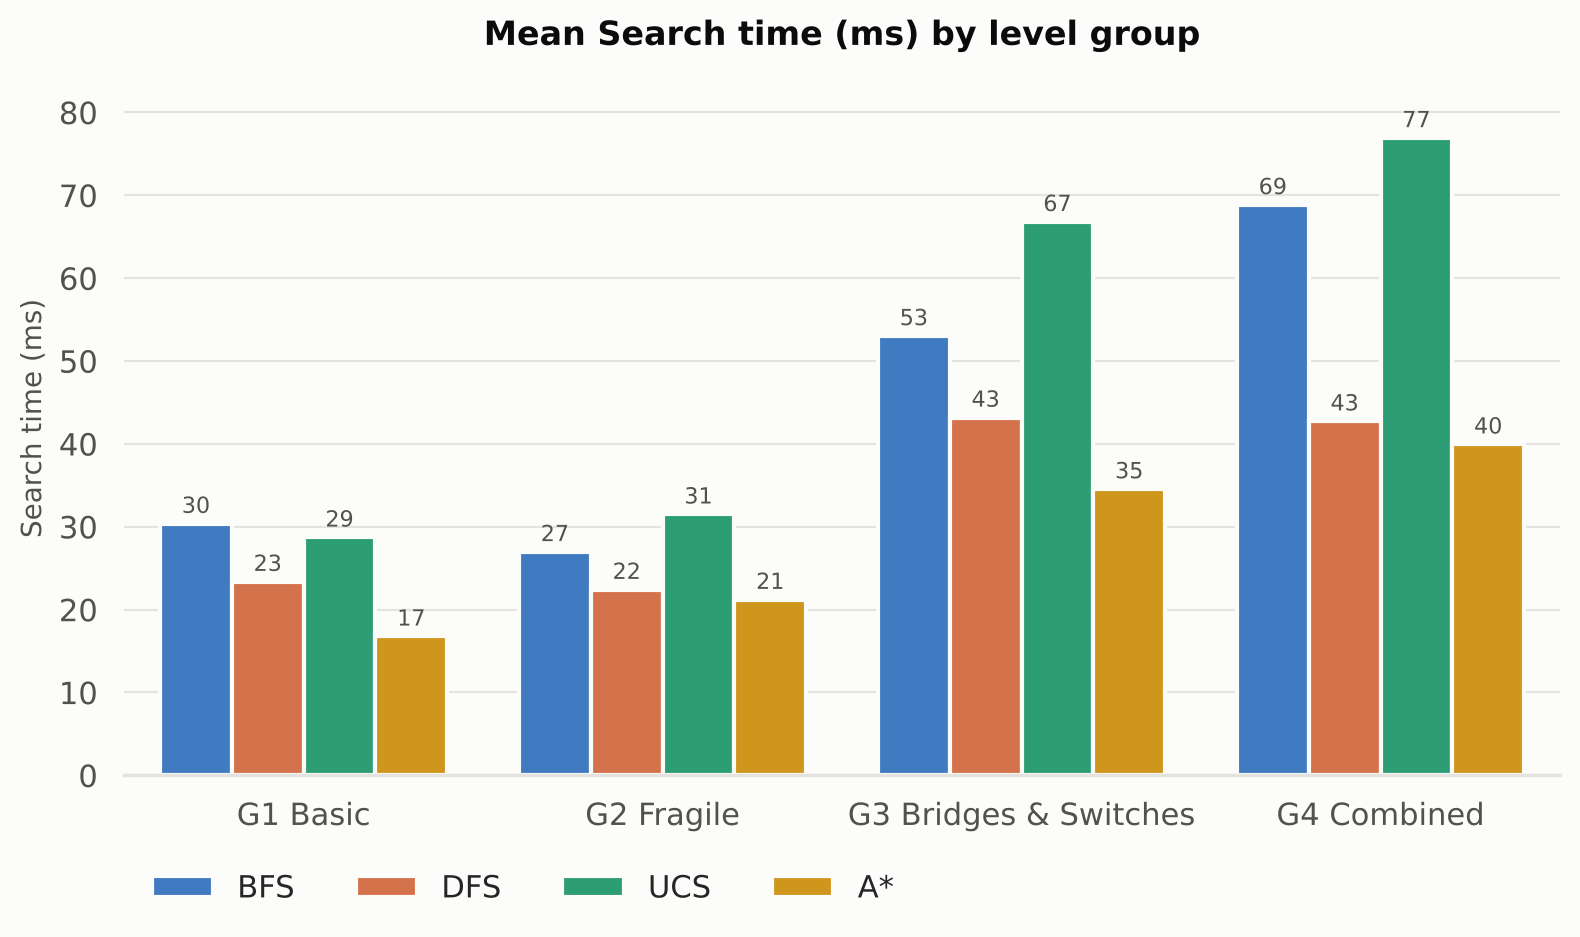
\includegraphics[width=\linewidth]{fig1a_time_by_group.png}
  \caption{Search time}
\end{subfigure}
\hfill
\begin{subfigure}{0.49\linewidth}
  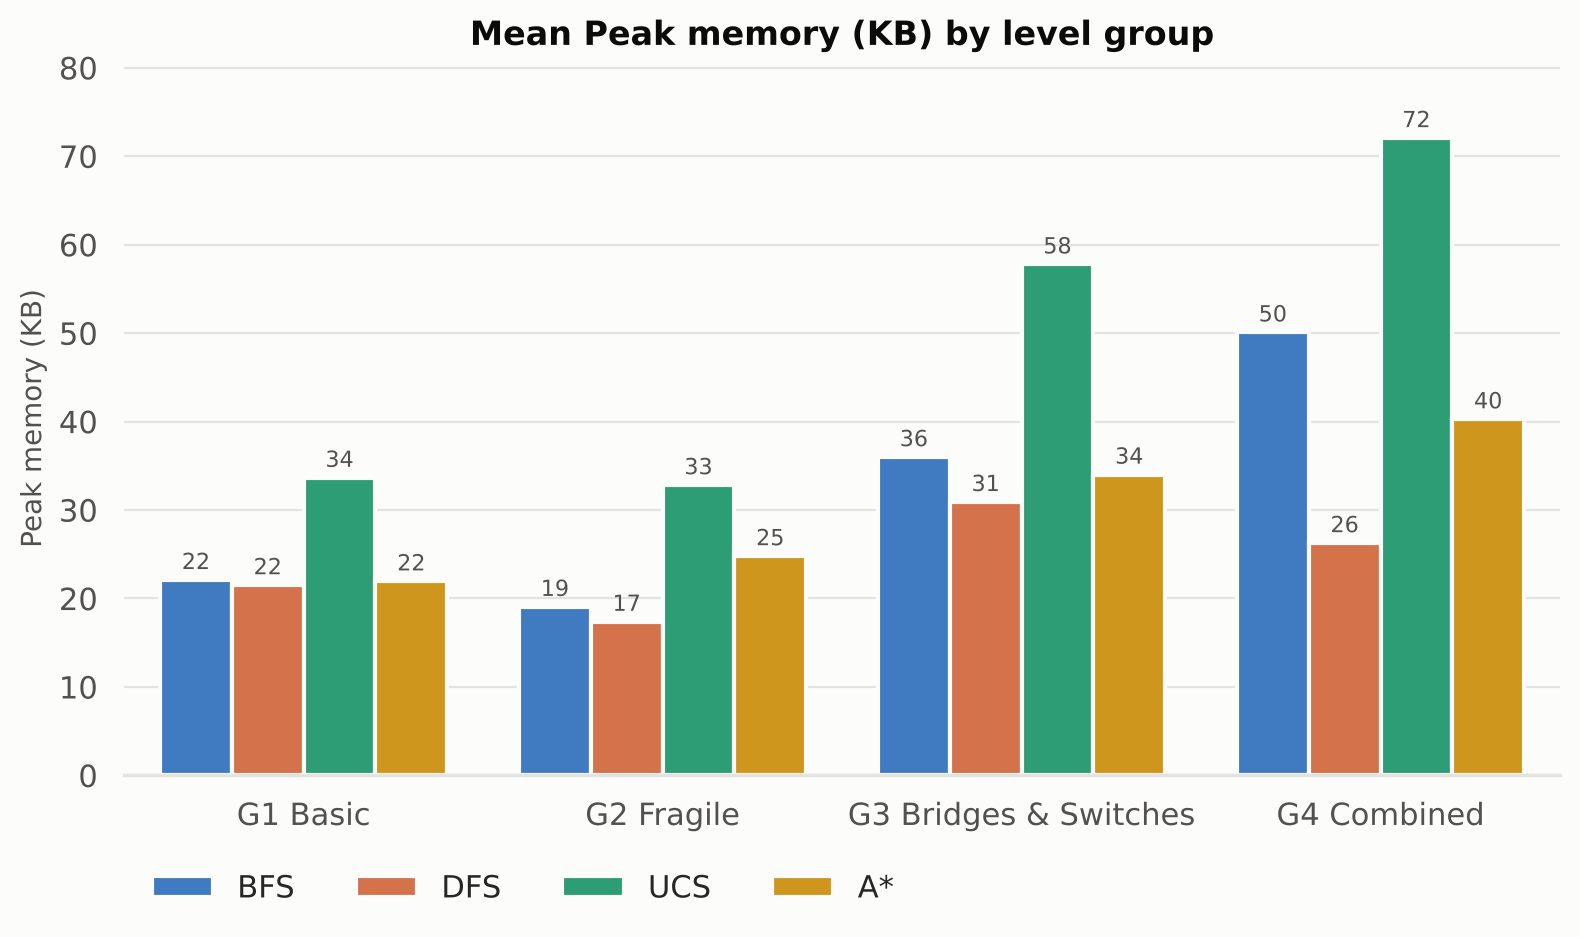
\includegraphics[width=\linewidth]{fig1b_memory_by_group.png}
  \caption{Peak memory}
\end{subfigure}
\\[0.3cm]
\begin{subfigure}{0.49\linewidth}
  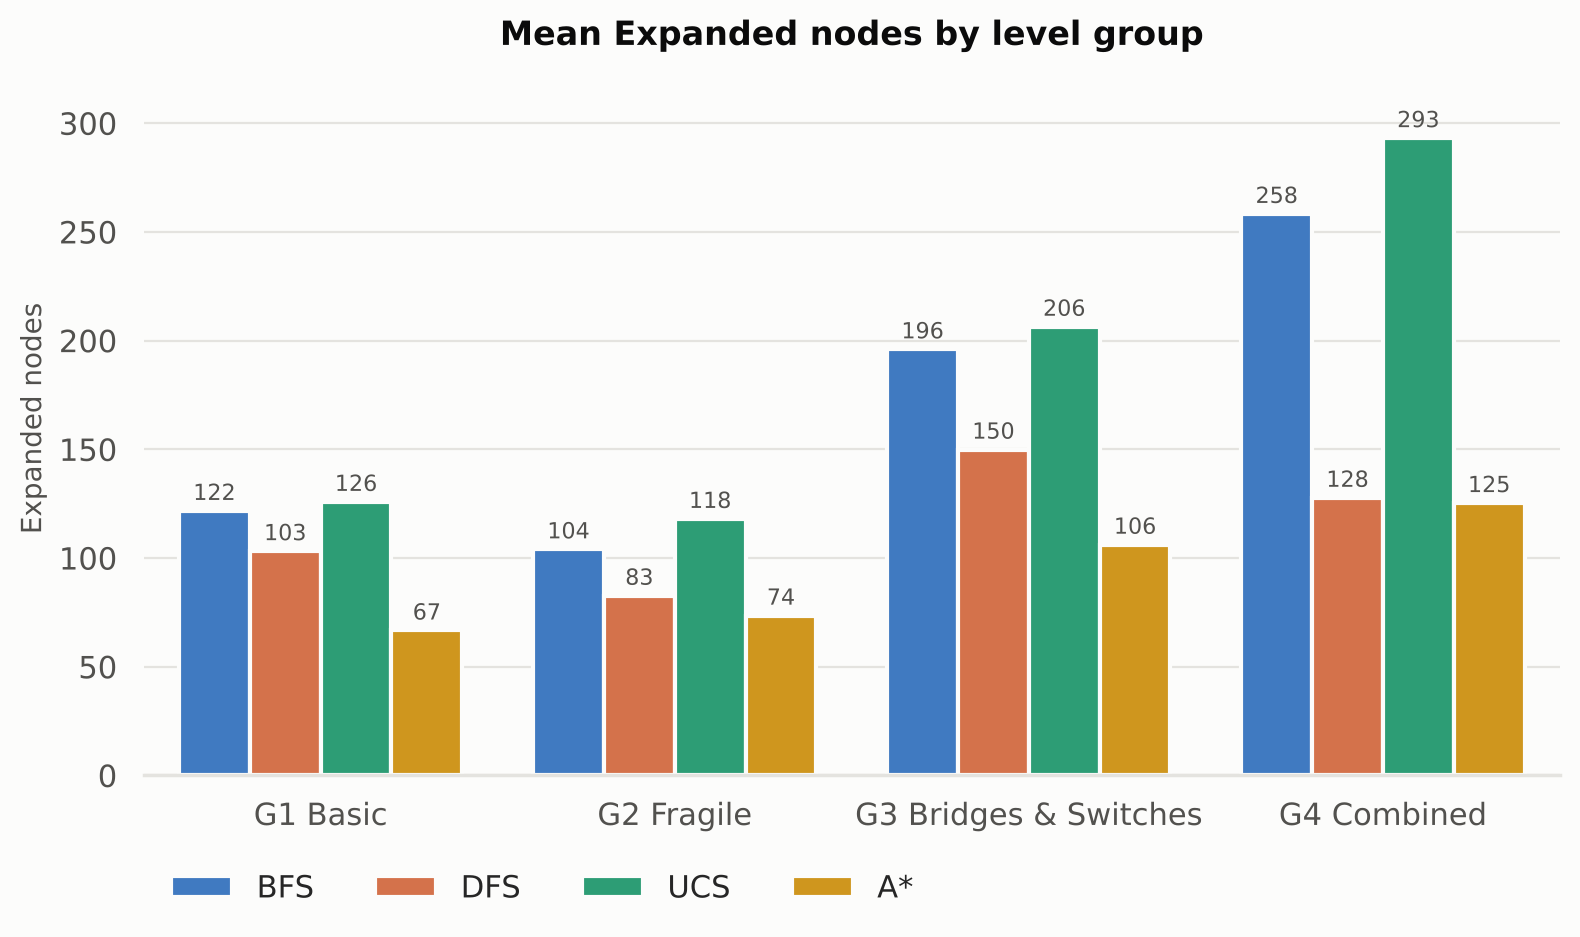
\includegraphics[width=\linewidth]{fig1c_expanded_by_group.png}
  \caption{Expanded nodes}
\end{subfigure}
\hfill
\begin{subfigure}{0.49\linewidth}
  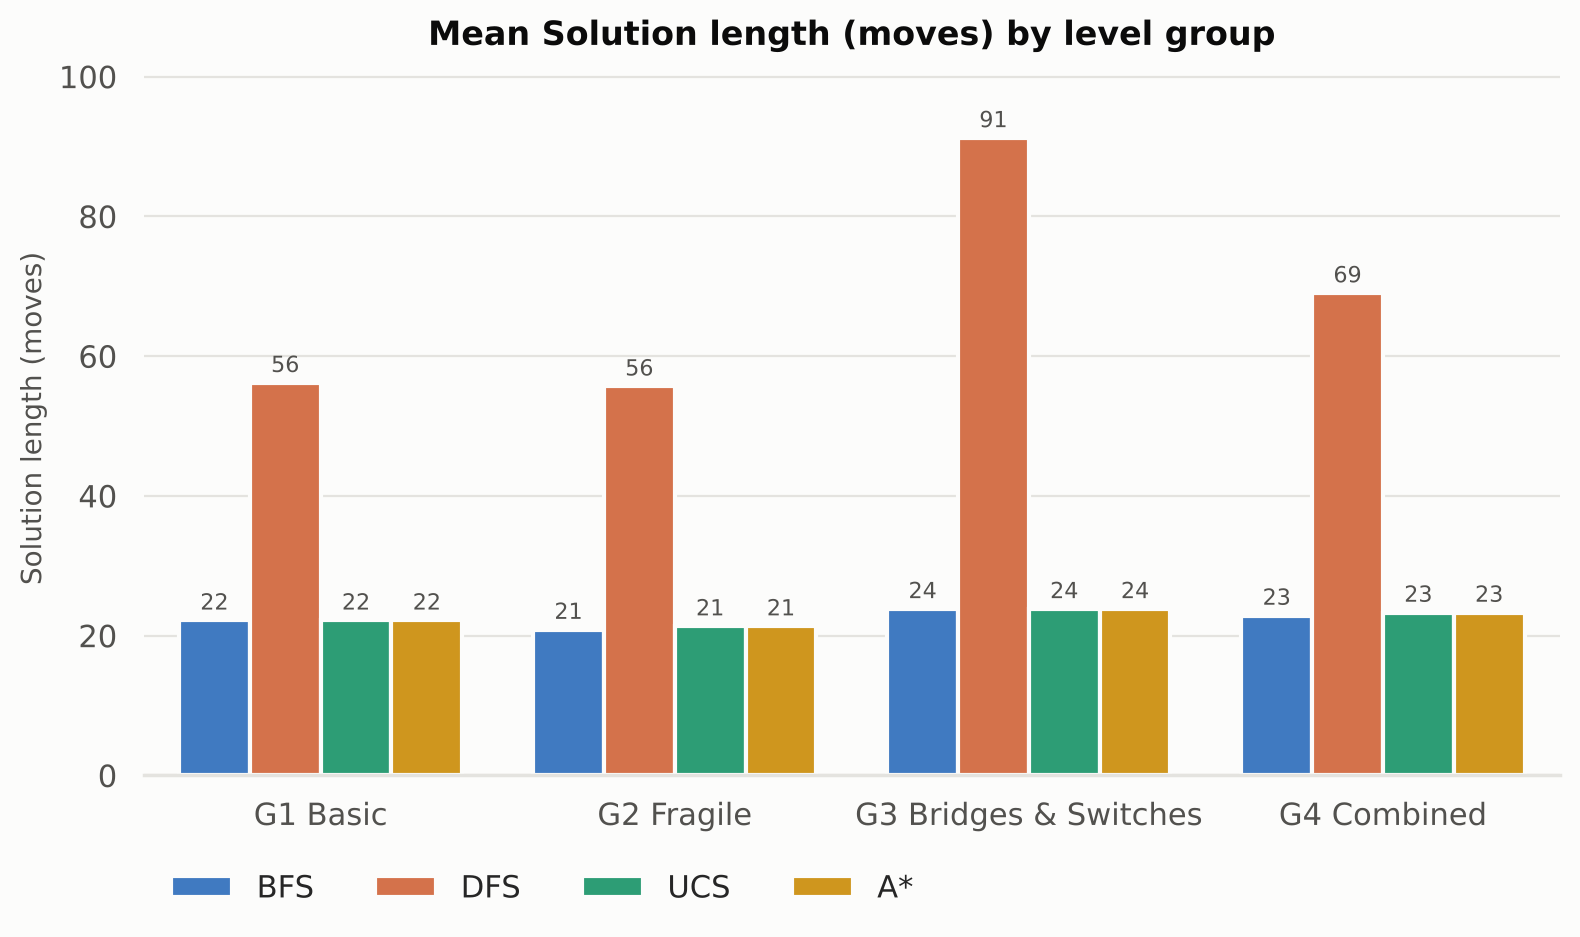
\includegraphics[width=\linewidth]{fig1d_moves_by_group.png}
  \caption{Solution length}
\end{subfigure}
\caption{Mean of the four metrics per test group}
\label{fig:groups}
\end{figure}

Figure~\ref{fig:groups}: from G1 to G4, the time, memory and expanded nodes of BFS and UCS roughly
double, because bridges multiply the state space by $2^B$. A* is lowest in time and expanded nodes
in every group. BFS, UCS and A* return solutions of almost the same length; DFS solutions are 2.5
to 4 times longer.

\begin{figure}[H]
\centering
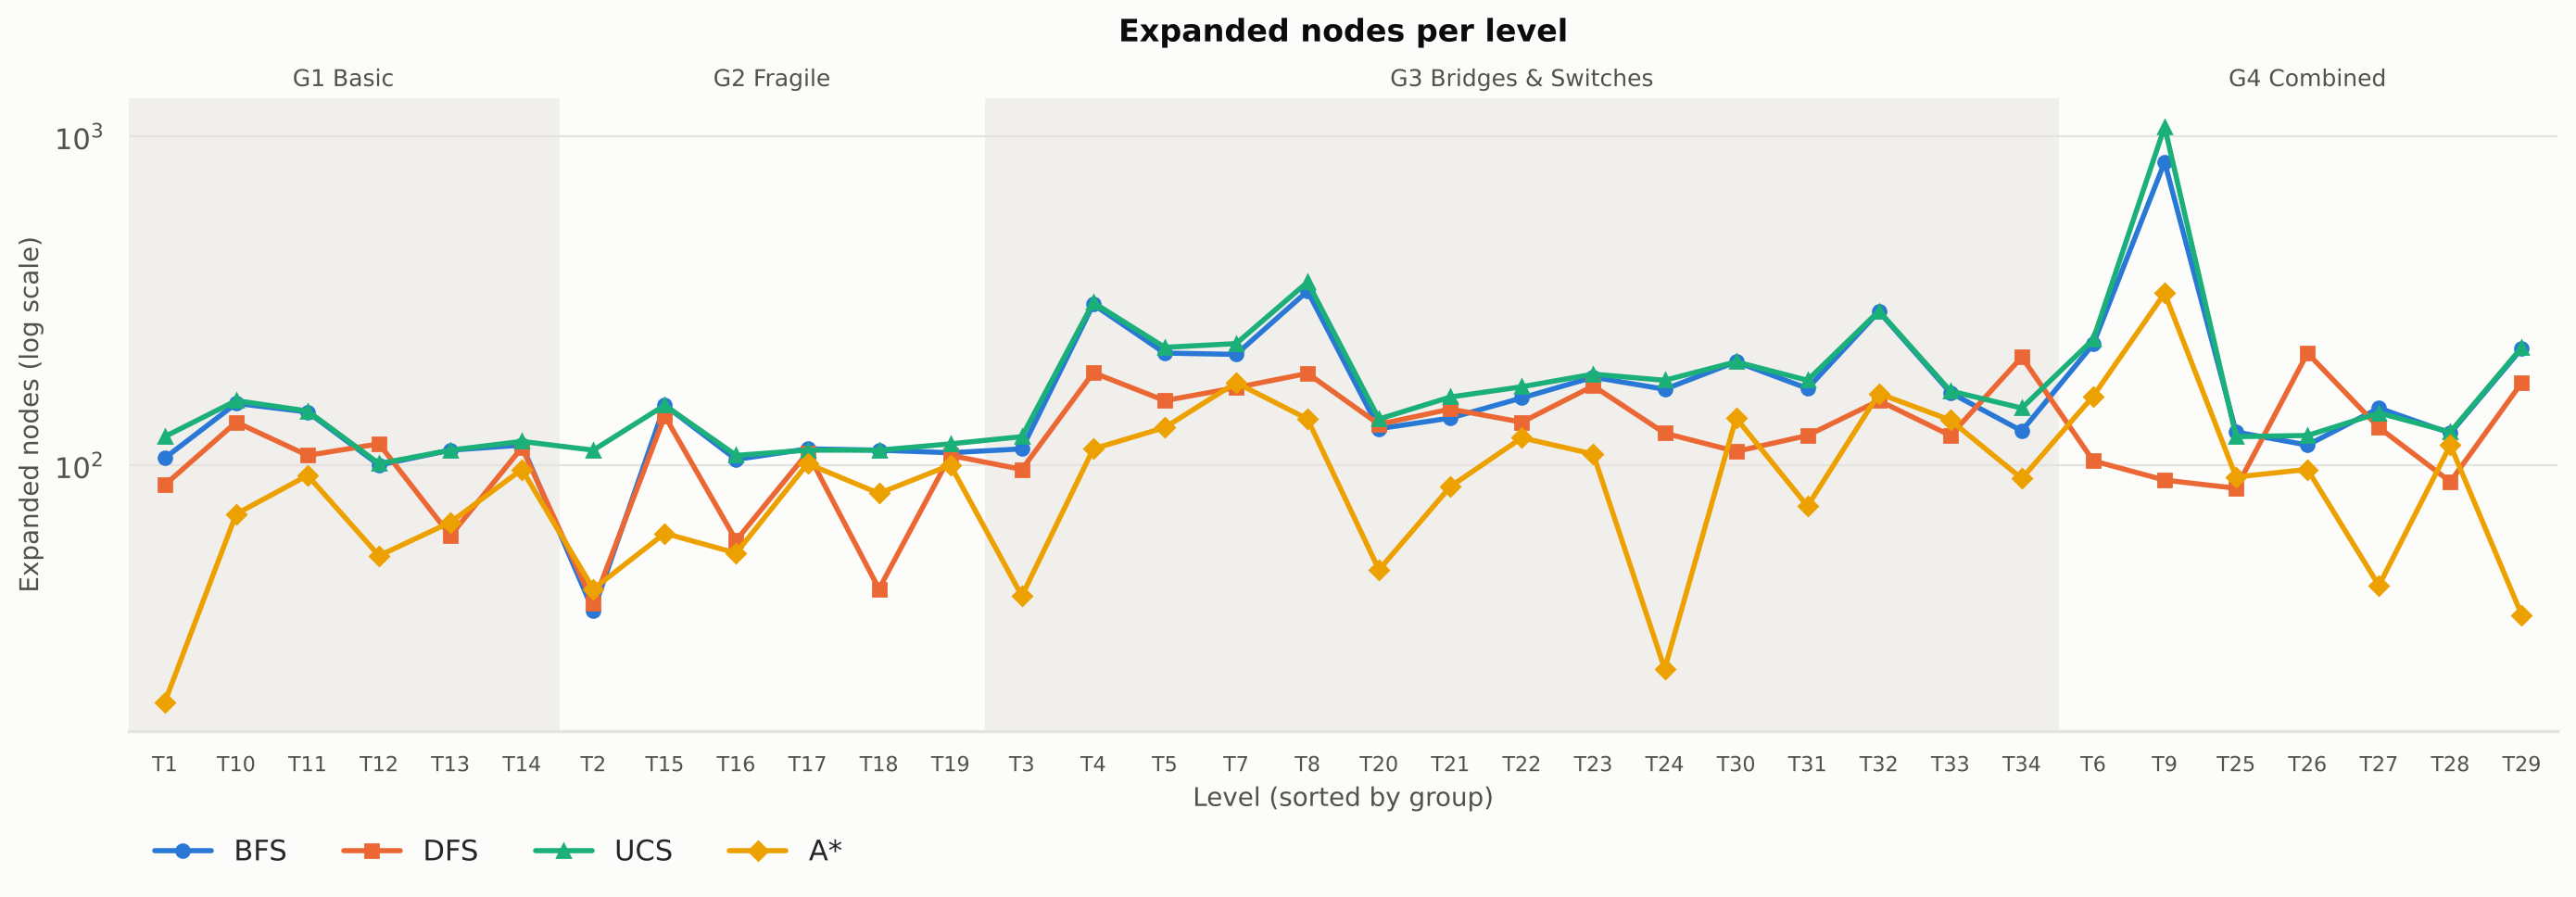
\includegraphics[width=\linewidth]{fig2_expanded_per_level.png}
\caption{Expanded nodes per stage (log scale), stages sorted by group}
\label{fig:perlevel}
\end{figure}

Figure~\ref{fig:perlevel}: the A* line lies below UCS on all 34 stages. BFS and UCS almost
coincide except on stages with fragile tiles. The largest peak is Test 9 (split switch), where BFS
and UCS expand 834 and 1068 states.

\begin{figure}[H]
\centering
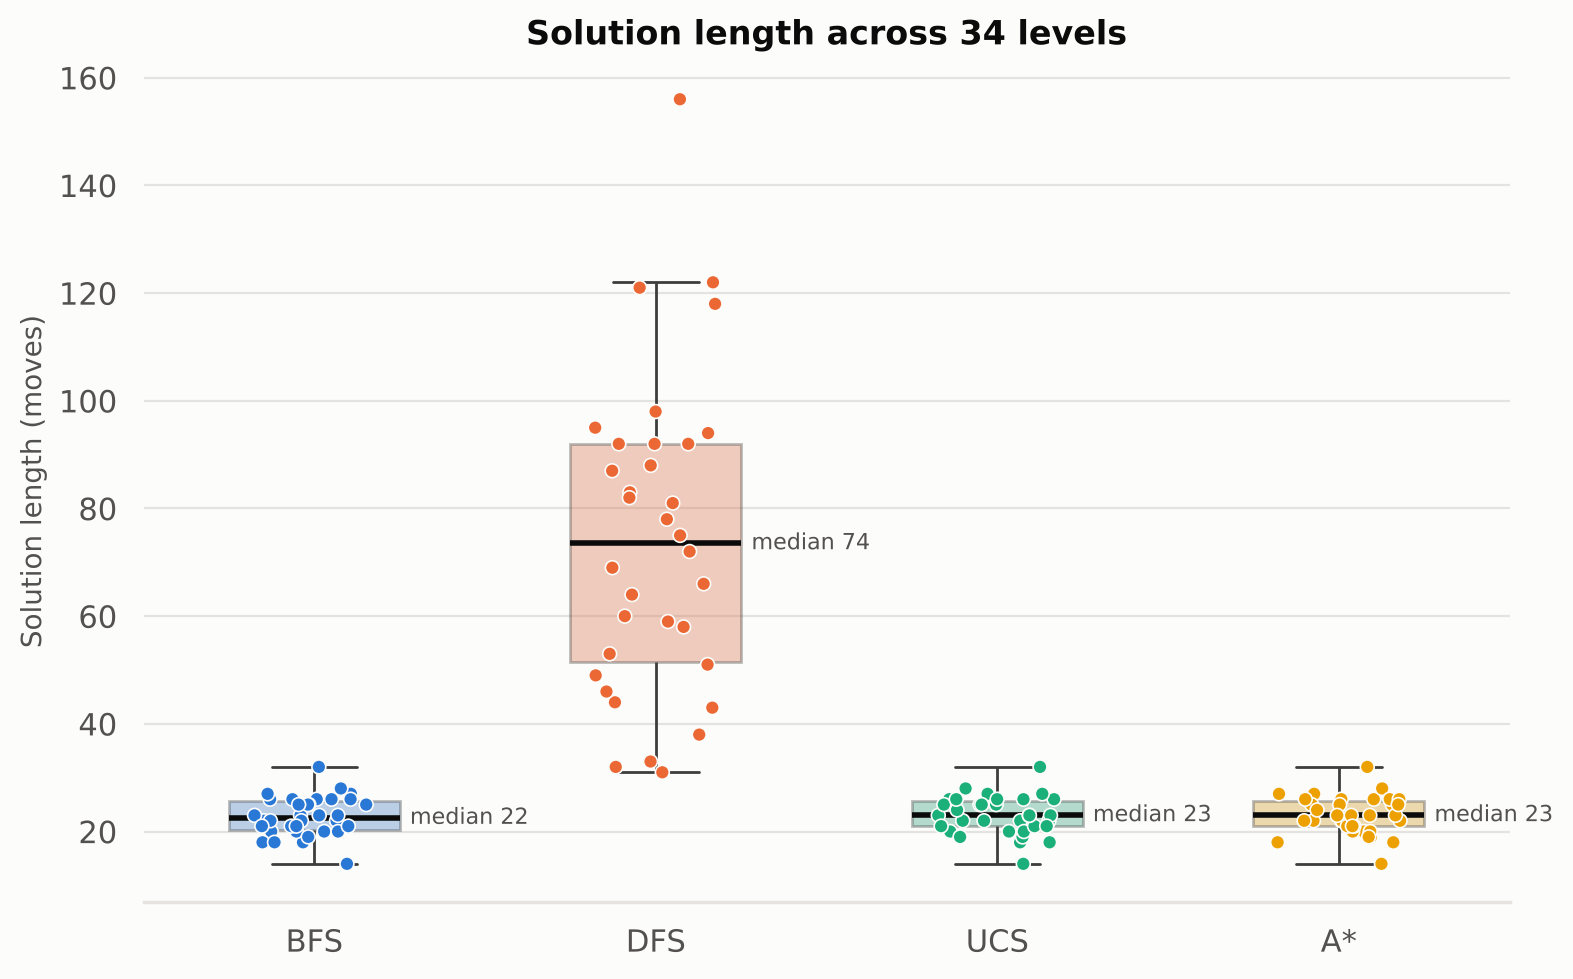
\includegraphics[width=0.75\linewidth]{fig3_moves_distribution.png}
\caption{Distribution of solution lengths over the 34 stages}
\label{fig:moves}
\end{figure}

Figure~\ref{fig:moves}: BFS, UCS and A* cluster around 22--23 moves, while DFS ranges from 31 to
156 moves (Test 4), with a median of 74.

\begin{figure}[H]
\centering
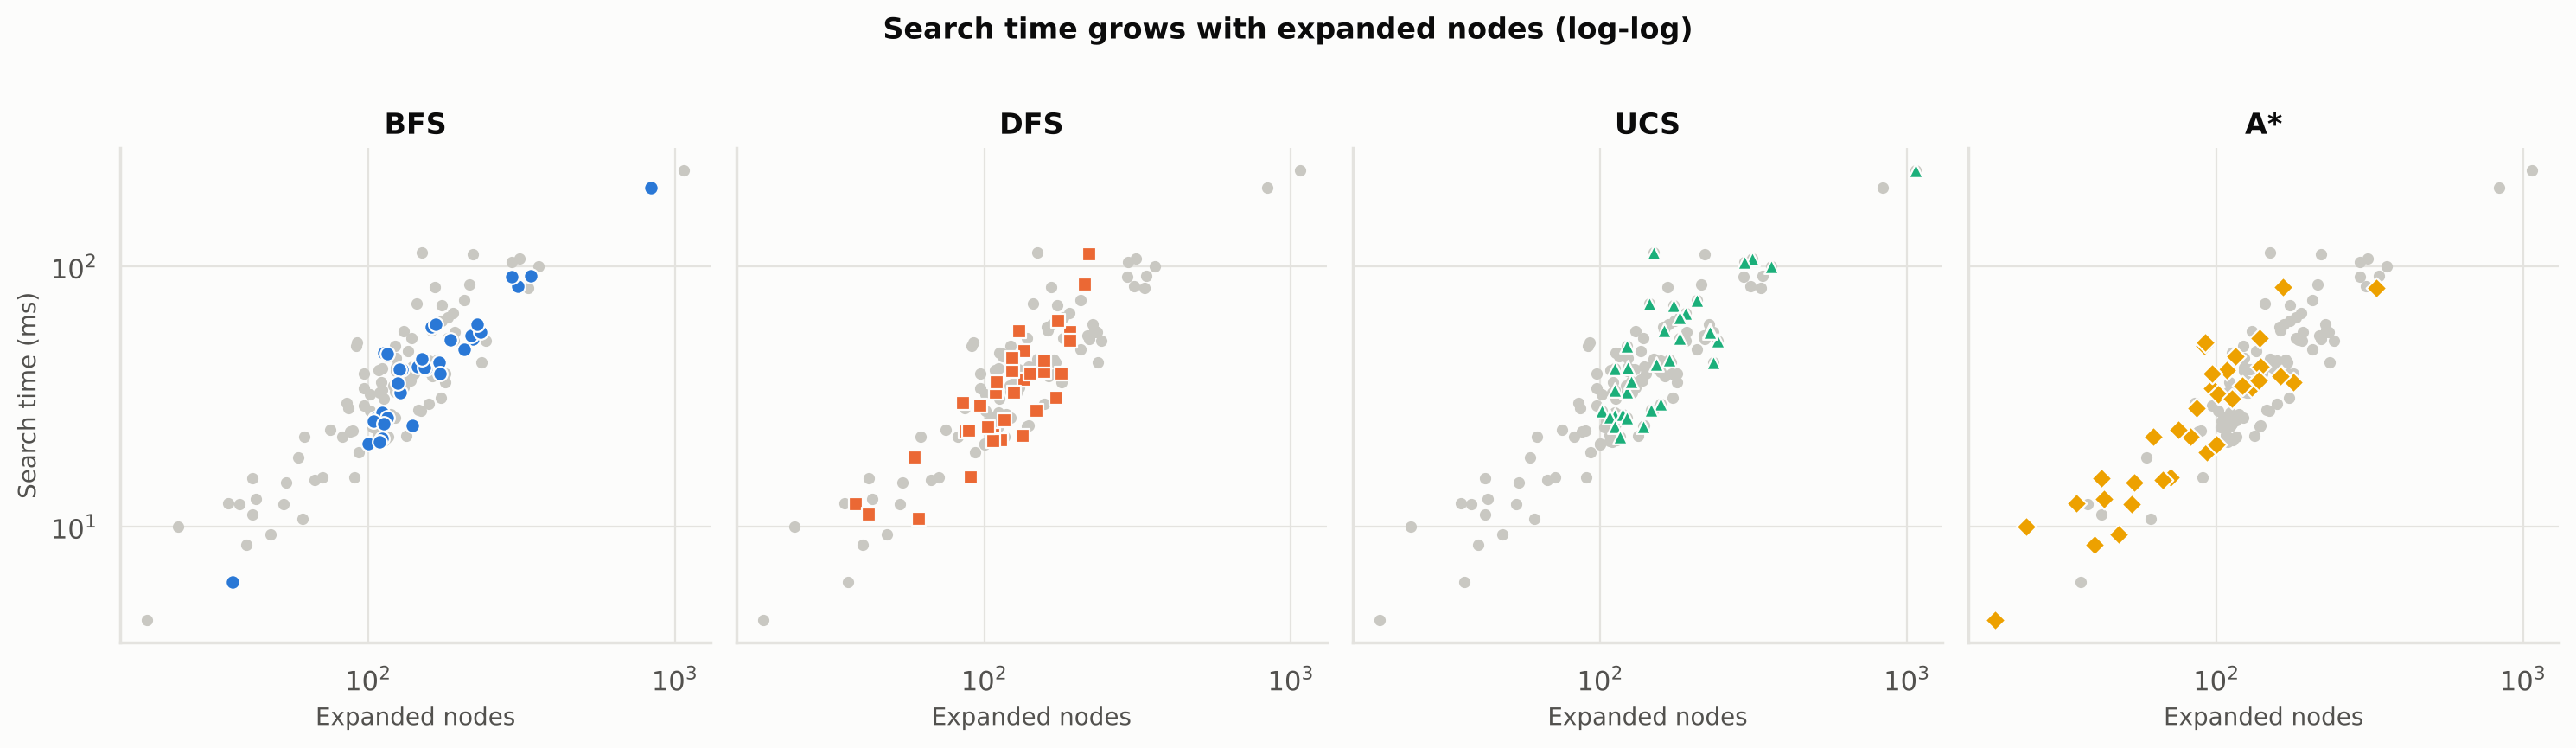
\includegraphics[width=\linewidth]{fig4_time_vs_expanded.png}
\caption{Search time against expanded nodes (log--log), one panel per algorithm}
\label{fig:timeexp}
\end{figure}

Figure~\ref{fig:timeexp}: the points lie close to a straight line (correlation 0.90 between log
time and log expanded nodes), so search time is driven mainly by the number of expansions. For the
same number of expansions, UCS and A* are slightly slower than BFS and DFS because each heap
operation costs $O(\log n)$ and A* also evaluates the heuristic.

\begin{figure}[H]
\centering
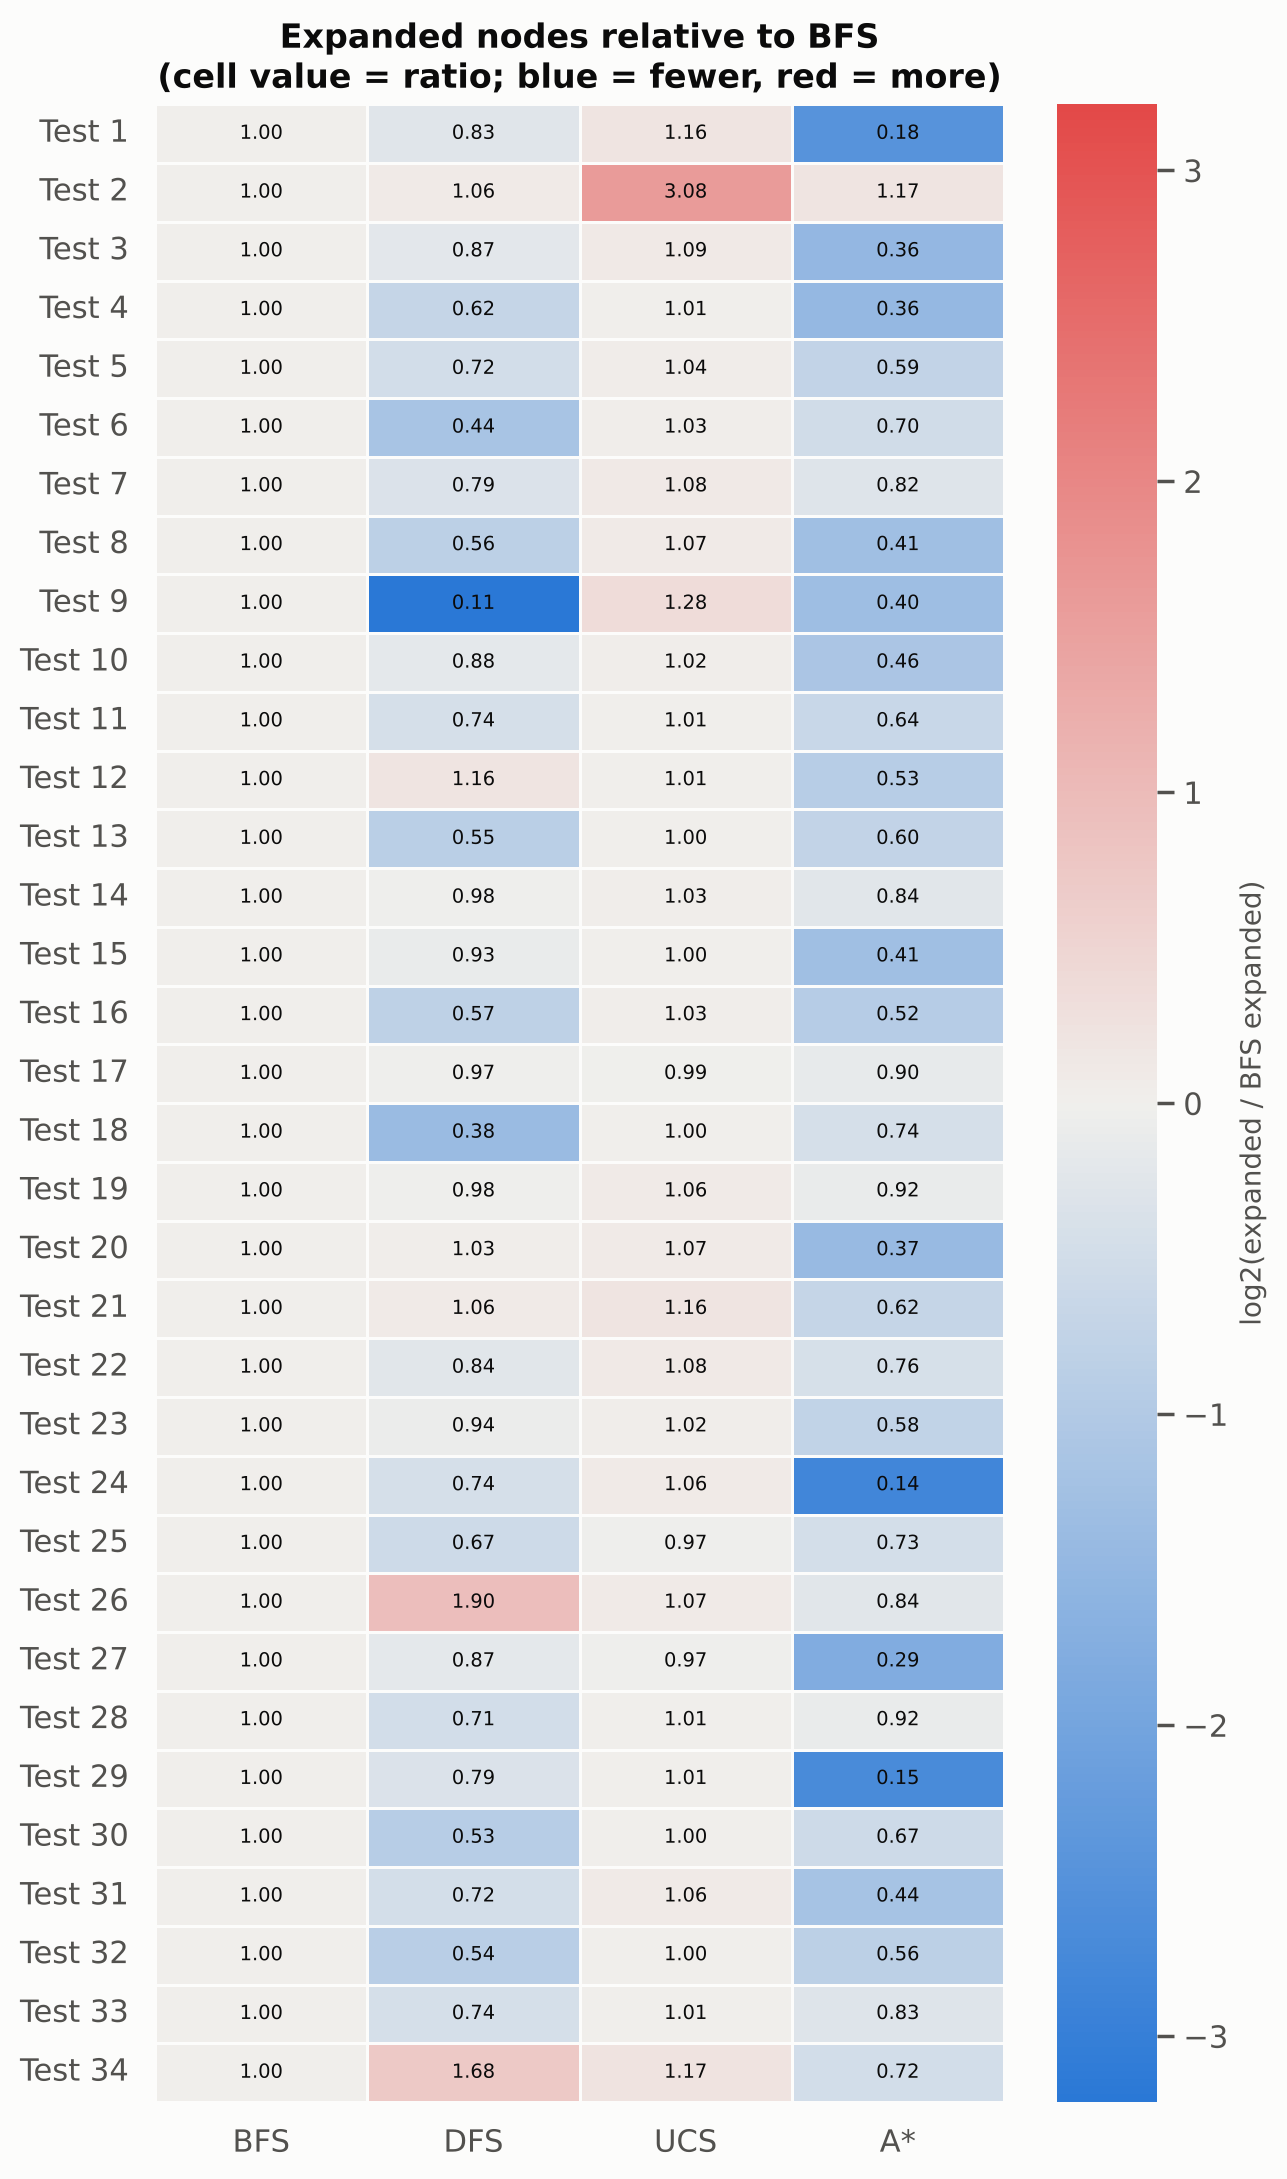
\includegraphics[width=0.62\linewidth]{fig5_expanded_ratio_heatmap.png}
\caption{Expanded nodes relative to BFS on the same stage (blue: fewer, red: more)}
\label{fig:heatmap}
\end{figure}

Figure~\ref{fig:heatmap}: A* expands fewer states than BFS on 33 of 34 stages (best: 0.14 on Test 24
and 0.18 on Test 1). UCS expands slightly more than BFS on 27 of 34 stages; Test 2 stands out with a
ratio of 3.08, explained in Section~\ref{sec:discussion}.

\begin{figure}[H]
\centering
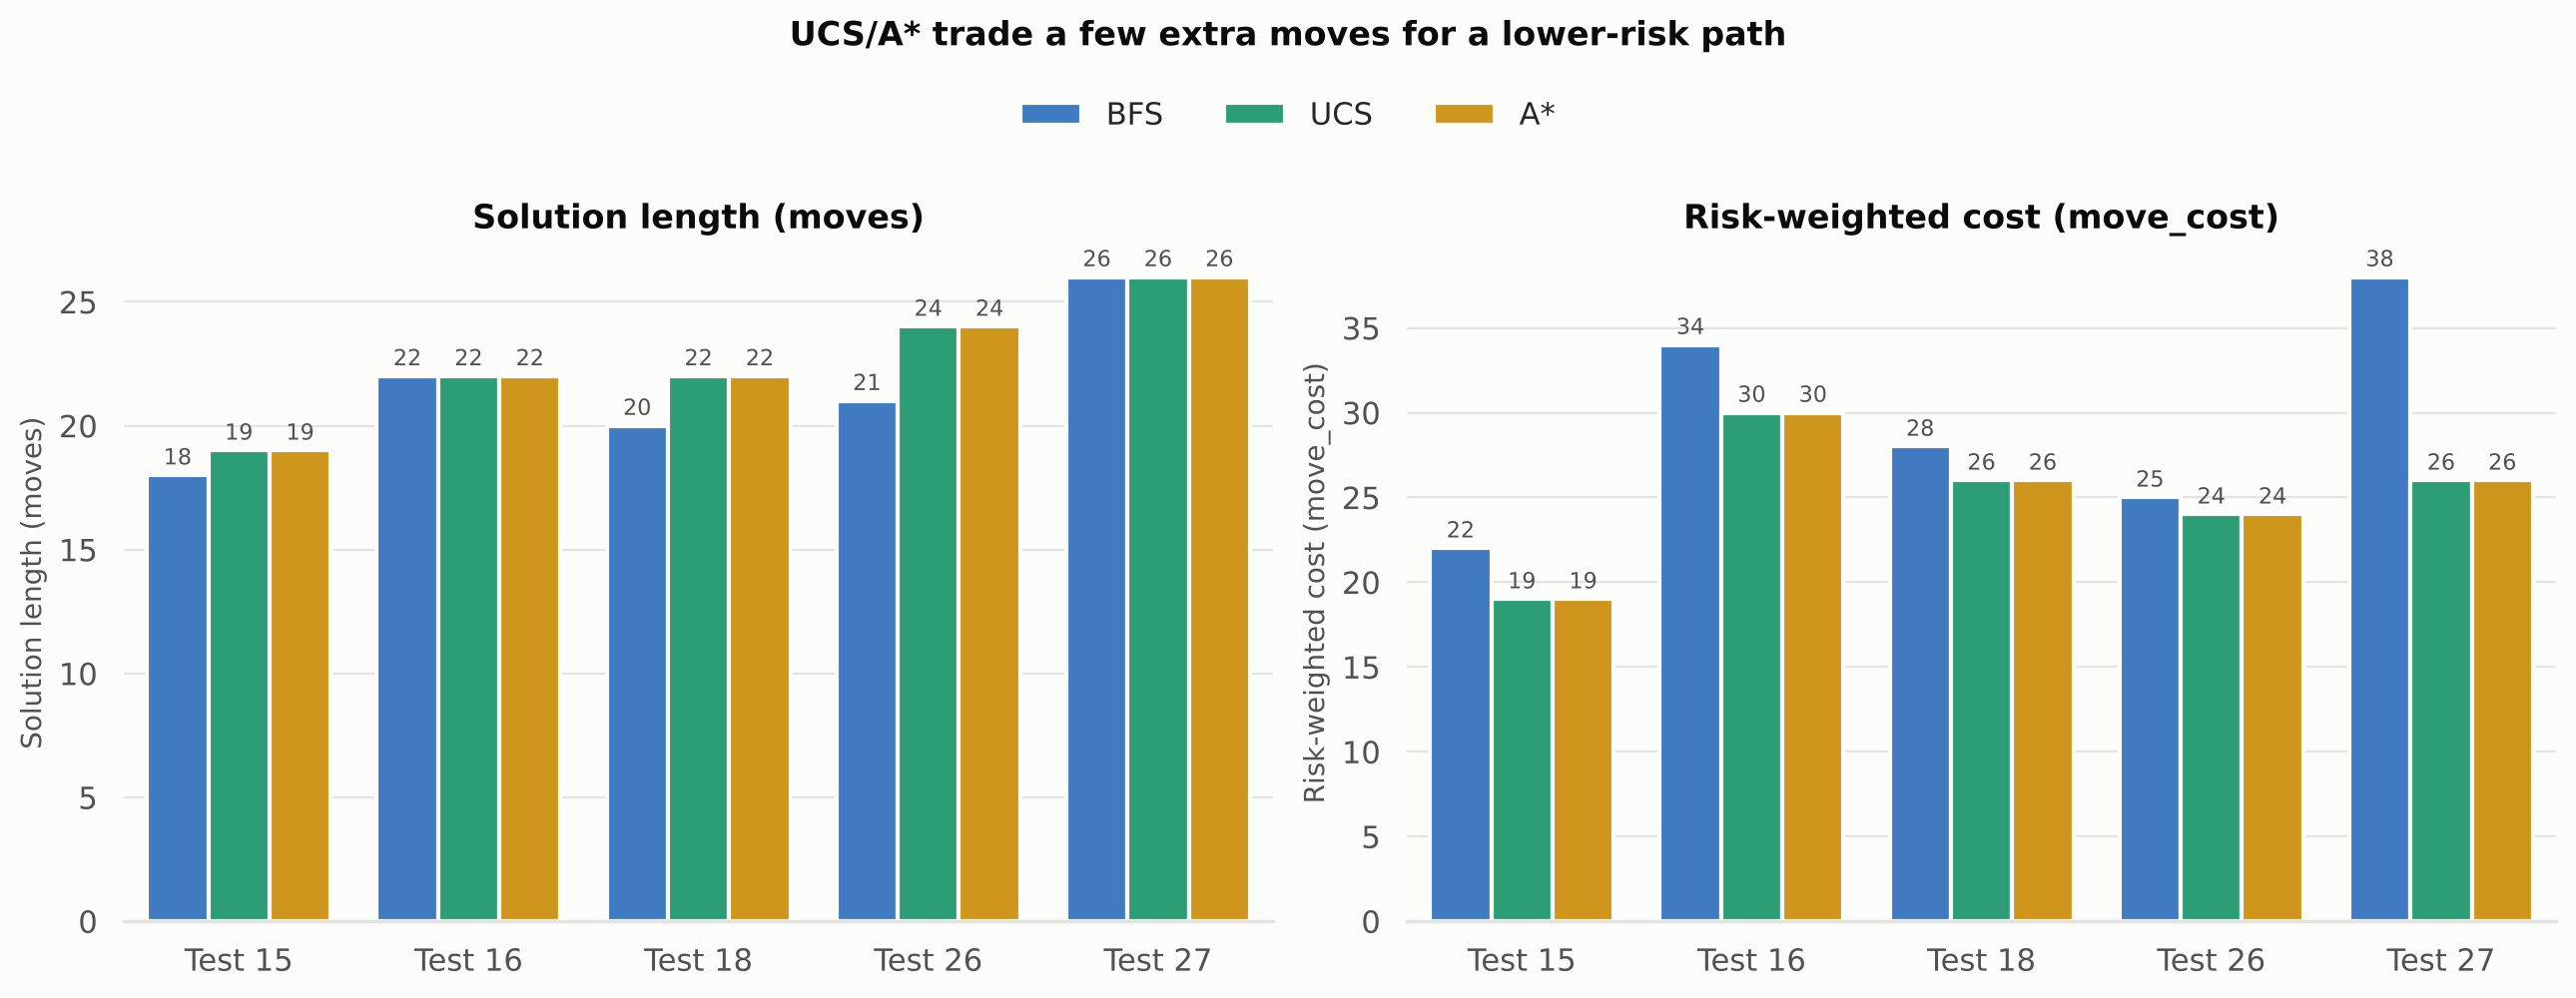
\includegraphics[width=\linewidth]{fig6_risk_tradeoff.png}
\caption{Stages where UCS/A* choose a different path from BFS: moves and risk cost}
\label{fig:risk}
\end{figure}

Figure~\ref{fig:risk}: on five stages UCS and A* pick a safer path than BFS. On Tests 15, 18 and 26
they take 1 to 3 extra moves to lower the risk cost; on Test 27 the path has the same 26 moves but
its cost drops from 38 to 26, avoiding all three fragile landings of the BFS path.

\subsection{Discussion}
\label{sec:discussion}

\textbf{Solution quality.} BFS, UCS and A* all return short solutions (22.8 to 23.0 moves on
average). UCS and A* return the same cost on all 34 stages, as theory predicts: both are optimal for
\texttt{move\_cost} and the heuristic is consistent. Compared with BFS they take only 0.18 extra
moves on average, but their risk cost is strictly lower on five stages (Tests 15, 16, 18, 26, 27).
On the other 29 stages the shortest path crosses no fragile tile, so any risk-based cost agrees
with BFS. DFS paths are on average 3.34 times longer than BFS paths (up to 7.1 times on a single
stage, and 1363 against 84 moves on Test All).

\textbf{Expanded nodes.} A* expands fewer states than UCS on every stage, 45\% fewer on average
(from 8.7\% on Test 28 to 86.7\% on Test 24). The heuristic helps most when the real path is close
to the straight line to the goal (Tests 1, 24, 29) and least on winding maps or around fragile tiles
(Tests 28, 17 and 19, only 9--14\% fewer). Over all four algorithms, A* expands the fewest states on 23 of
34 stages. UCS expands more than BFS on 27 stages for two reasons: BFS stops when the goal is
\emph{generated} while UCS waits until it is \emph{popped}, and the fragile penalty widens UCS's cost
contours. Test 2 is the extreme case: its solution must cross a fragile tile (cost 22 for 18 moves),
so UCS has to expand every state cheaper than 22, including states 19 to 21 moves deep that BFS never
reaches (111 against 36 expansions). DFS expands fewer states than BFS on 28 stages because it dives
deep and meets the goal early, at the price of very long paths.

\textbf{Time.} Time follows expanded nodes (Figure~\ref{fig:timeexp}). On average A* is fastest
(30 ms, fastest on 20 of 34 stages), then DFS (36 ms), BFS (48 ms) and UCS (56 ms). On Test All, DFS
is fastest (138 ms) because it expands the fewest states, and A* is second (188 ms).

\textbf{Memory.} UCS uses the most memory (highest on 32 of 34 stages): besides \texttt{parents} it
keeps \texttt{best}, \texttt{closed} and a heap that also holds stale entries. A* keeps the same
structures but expands far fewer states, so its memory is close to BFS. DFS uses the least memory on
16 of 34 stages. On Test All: UCS 2.5 MB, BFS 1.4 MB, A* 0.9 MB, DFS 0.8 MB.

\textbf{Effect of difficulty.} Bridges and switches (G3, G4) increase the work more than fragile
tiles (G2): each bridge group doubles the number of possible configurations, whereas fragile tiles
only forbid some standing placements. Split switches (Test 9, Test All) create the largest state
spaces because the two cubes move independently.

\begin{table}[H]
\centering
\caption{Strengths and weaknesses}
\label{tab:proscons}
\begin{tabularx}{\linewidth}{lXX}
\toprule
\textbf{Algorithm} & \textbf{Strengths} & \textbf{Weaknesses} \\
\midrule
BFS & Simple; optimal in the number of actions; stops as soon as the goal is generated & Ignores risk; expands and stores many states; not move-optimal when \texttt{SWAP} is used \\
DFS & Fewer expansions than BFS on 28/34 stages; least memory on 16/34; fastest on Test All & Solutions 3.3 times longer on average (16 times on Test All); result depends on the order in which actions are tried \\
UCS & Optimal for any non-negative cost; needs no heuristic; avoids fragile tiles & Slowest and most memory-hungry; extra expansions when the solution is expensive \\
A* & Same optimal cost as UCS with about 45\% fewer expansions; fastest on average & Needs a carefully designed and proven heuristic; weak on winding maps \\
\bottomrule
\end{tabularx}
\end{table}

\subsection{Limitations}

\begin{itemize}[leftmargin=*]
\item Each configuration was run once; averaging several runs would reduce timing noise.
\item \texttt{tracemalloc} slows Python down, so absolute times are higher than in the GUI.
\item The generated stages have similar sizes ($12\times25$) and goals usually on the right; Test All
complements them with a much larger map.
\item All runs start from the stage's initial state, not from mid-level states.
\end{itemize}
